\documentclass[10pt,letterpaper]{article}
\usepackage{mathpazo}
\usepackage[scaled]{helvet}
\usepackage[T1]{fontenc}
\usepackage{hyperref}
\usepackage{color,soul}
\usepackage{graphicx}
\usepackage[justification=centering,singlelinecheck=false]{caption}
%\usepackage{setspace}
\usepackage[margin=1in,includehead,includefoot]{geometry}
\usepackage[table,dvipsnames]{xcolor}
\usepackage{amssymb}
\usepackage{amsmath}
\usepackage{fancyhdr}
\usepackage{array}
\usepackage{gensymb}
\usepackage{lastpage}
\usepackage{textcomp}
\usepackage{booktabs}
\usepackage{pdfpages}
\usepackage{tabto}
\usepackage{multicol}
\usepackage{tabularx}
\usepackage{framed}
\usepackage{chngcntr}
\usepackage{tocloft}
\usepackage[font={sf,normalsize},labelfont={sf,bf}]{caption}
\usepackage{float}
\usepackage{tikz}
\usepackage{listings}
\lstset{basicstyle=\small\ttfamily,breaklines=true}
\usepackage{forest}
\usepackage{verbatim}
\usepackage{longtable}
\usepackage{tabu}
\usepackage{afterpage}
\usepackage{paralist}
\usepackage{indentfirst}
\usepackage{changepage}

\newenvironment{Figure}
{\par\medskip\noindent\minipage{\linewidth}}
{\endminipage\par\medskip}

%% no indentation
%\setlength{\parindent}{0pt}

%%header and footer
\fancyhf{}
\renewcommand{\footrulewidth}{0pt}
\renewcommand{\headrulewidth}{0pt}
\rhead{\nouppercase{\leftmark}}
\lhead{\sf \textbf{Project 2}  |  Reinforcement Learning}
\rfoot{\sf \textbf{0\thepage} OF \textbf{0\pageref*{LastPage}}}
\rhead{\sf \textbf{AA 228} | Decision Making Under Uncertainty}
\pagestyle{fancy}


%% DOCUMENT START --------------------------------------------------

\begin{document}
		
	\captionsetup[figure]{labelformat=simple, labelsep=quad, labelfont={sf, bf}}
	\captionsetup[table]{labelformat=simple, labelsep=quad, labelfont={sf, bf}}
	
	\section*{\sf \textbf{Reinforcement Learning}}
	\vspace*{-0.1 in}
	{\noindent \sf \large R. B. Alexander}
	
	\vspace*{0.2 in}
	
\begin{adjustwidth}{1cm}{1cm}
		
	\noindent \textbf{}%Abstract text.}
	
\end{adjustwidth}
					
	\subsection*{\sf \textbf{Subsection 1}}
	
	\subsection*{\sf \textbf{Subsection 2}}
	
	\subsubsection*{\sf \textbf{Subsubsection 2.1}}
		
	\subsection*{\sf \textbf{Subsection 3}}

%	\begin{center}
%		\captionof{table}{Runtimes in Seconds for K2 Search with Randomized Start}
%		\vspace*{10pt}
%		\label{tab:runtime}
%		\begin{tabular}{l|l|l|l|l|}
%			\cline{2-5}
%			&                                                  \multicolumn{4}{c|}{\textbf{Iterations}}                                                   \\ \hline
%			\multicolumn{1}{|l|}{\textbf{Dataset}} & \multicolumn{1}{c|}{\textit{1}} & \multicolumn{1}{c|}{\textit{10}} & \multicolumn{1}{c|}{\textit{100}} & \multicolumn{1}{c|}{\textit{1000}} \\ \hline
%			\multicolumn{1}{|l|}{\texttt{small}}   & 3.1187                        & 16.341                         & 104.40                          & 1002.7                           \\ \hline
%			\multicolumn{1}{|l|}{\texttt{medium}}  & 29.534                        & 249.30                         & 2516.8                          & \cellcolor[HTML]{EFEFEF}           \\ \hline
%			\multicolumn{1}{|l|}{\texttt{large}}   & 8219.9                        & \cellcolor[HTML]{EFEFEF}         & \cellcolor[HTML]{EFEFEF}          & \cellcolor[HTML]{EFEFEF}           \\ \hline
%		\end{tabular}
%	\end{center}

%	\begin{figure*}[h!]
%		\centering
%		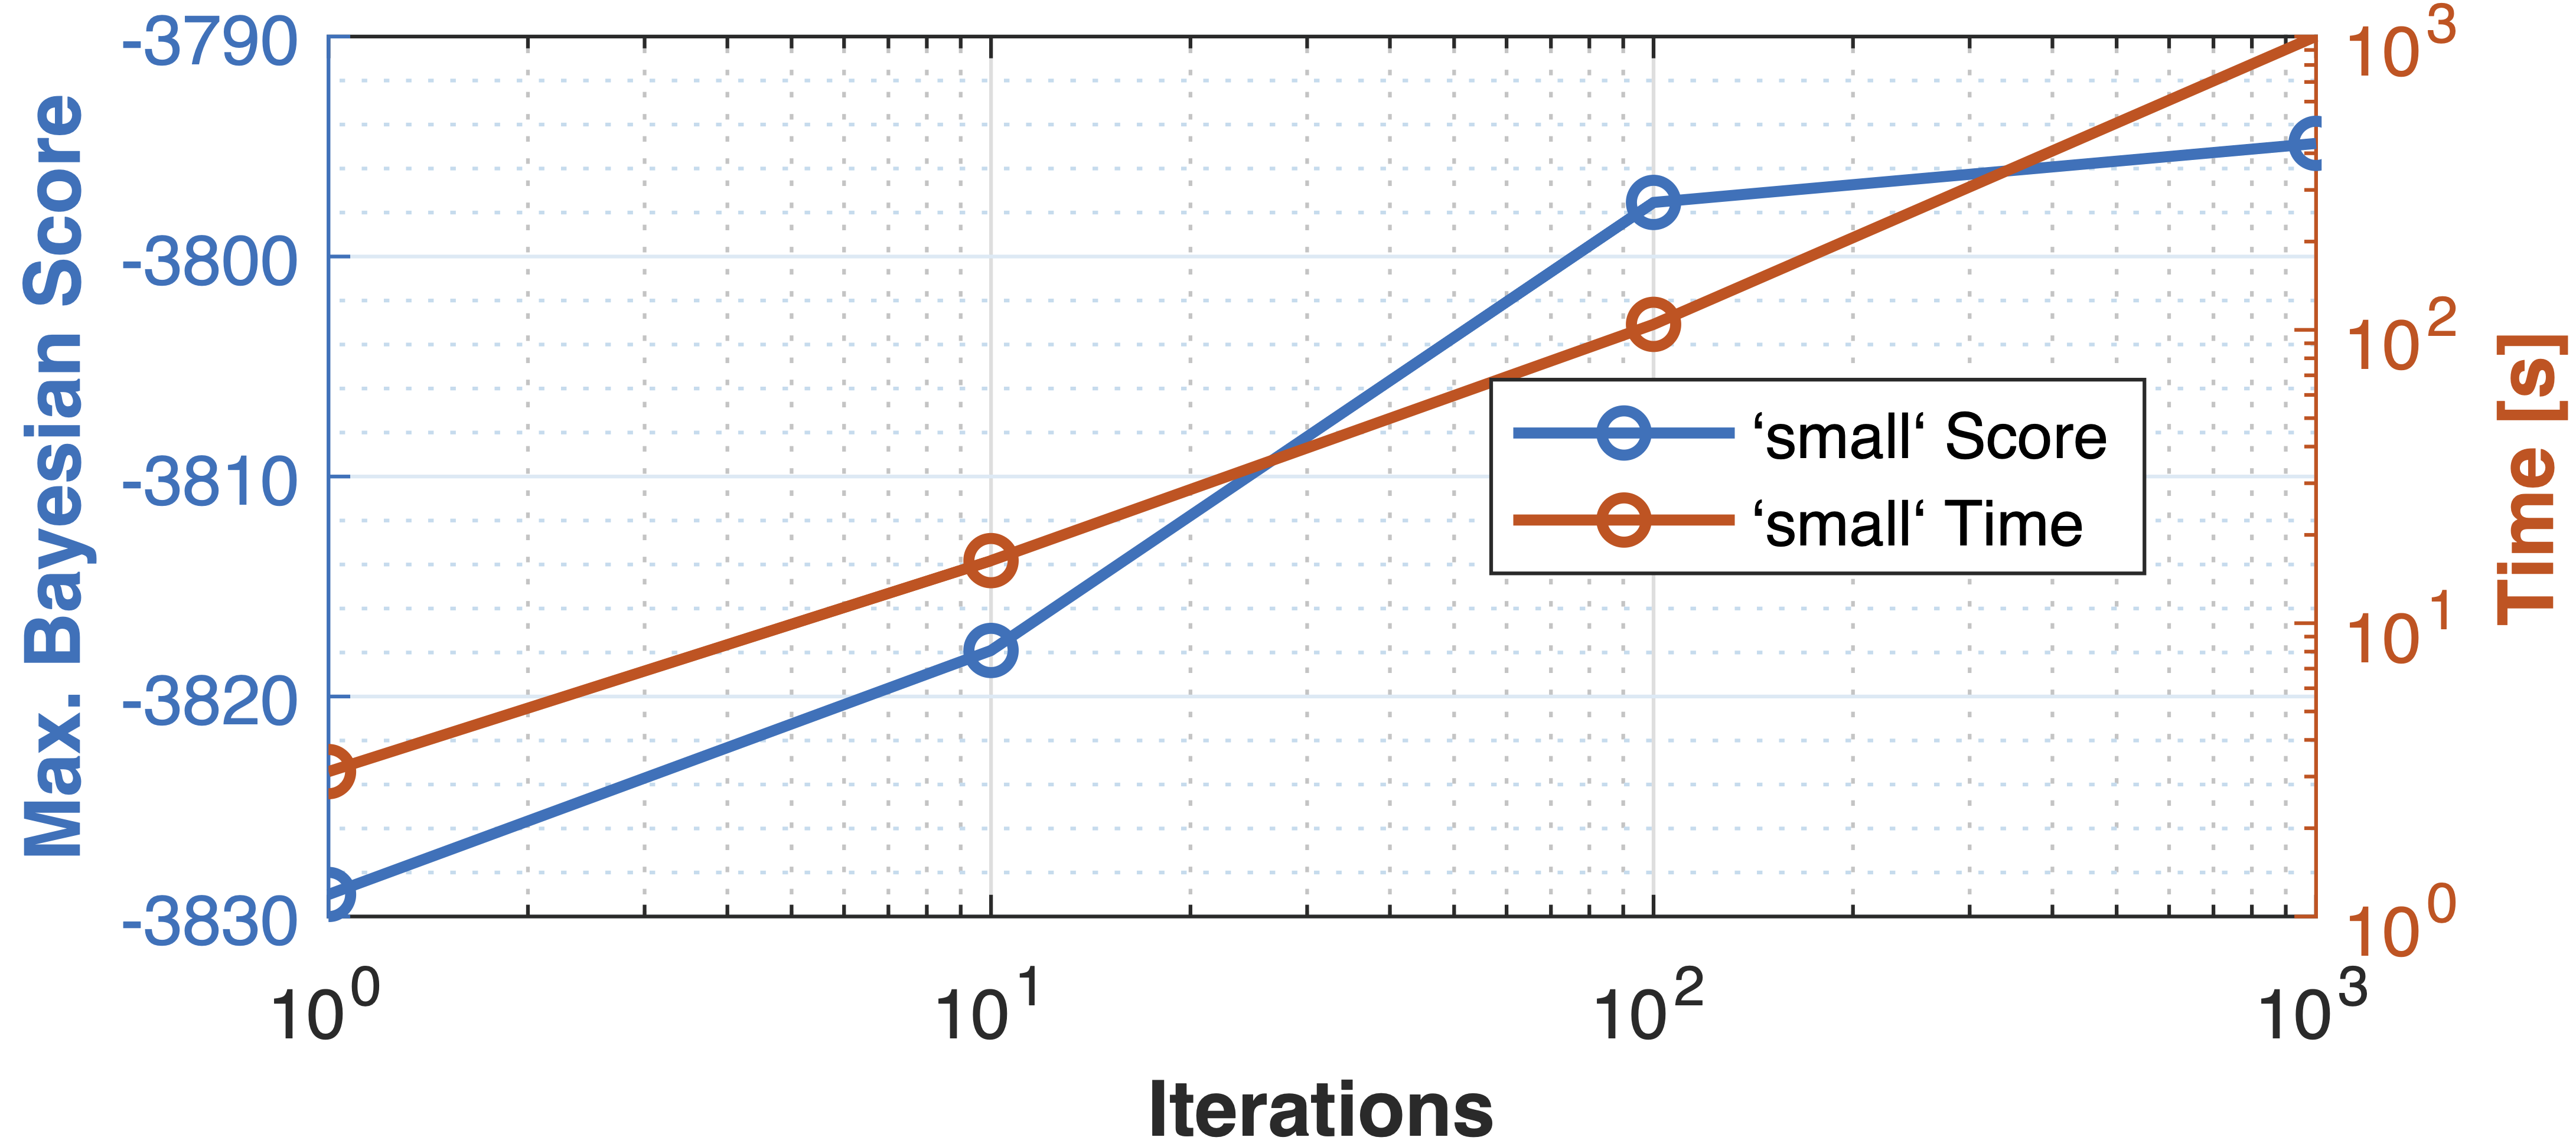
\includegraphics[width=0.47\linewidth]{figs/small-score-time.png}
%		\hspace*{0.15 in}
%		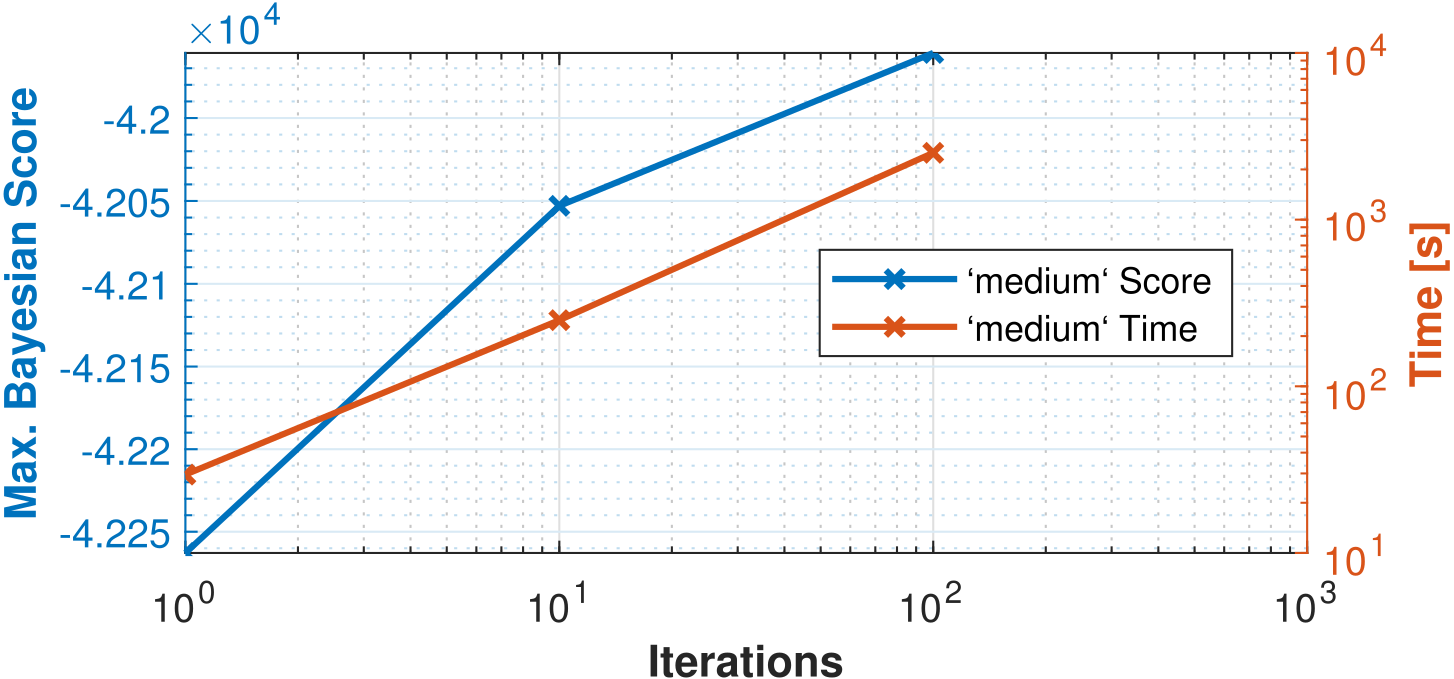
\includegraphics[width=0.47\linewidth]{figs/medium-score-time.png}
%		\setlength{\belowcaptionskip}{-10pt}
%		\captionof{figure}{Bayesian score improvement using K2 search iterated over randomly-permuted variable orderings for the \texttt{small} (\textit{left}) and \texttt{medium} (\textit{right}) datasets.}
%		\label{fig:time_score_graph}
%	\end{figure*}

%\begin{multicols}{2}
%	\begin{Figure} %[t]
%		\centering
%		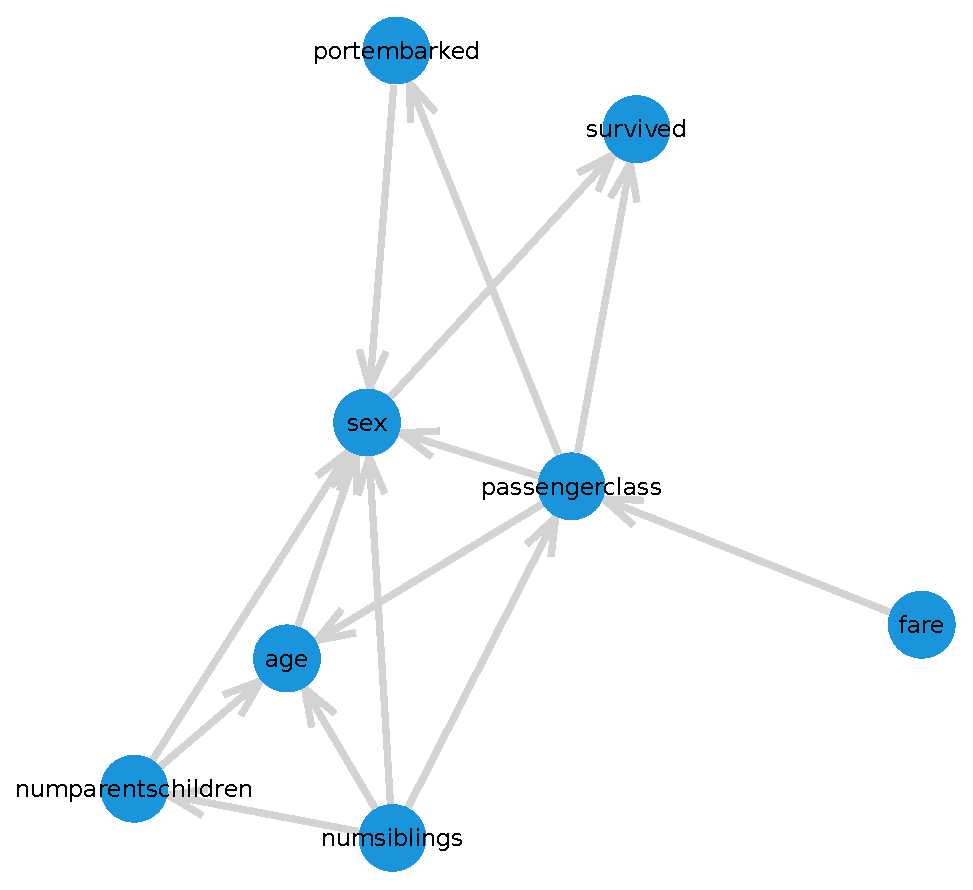
\includegraphics[height=0.33\textheight]{figs/small-K2-1000}
%				\setlength{\belowcaptionskip}{-10pt}
%		\captionof{figure}{\sf Bayesian network learned from the \texttt{small} dataset (8 variables) using a K2 search of the space of directed acyclic graphs with 1000 randomized starts. ($\ln P(G\mid D) \approx -3795 $)}
%		\label{fig:small_graph}
%	\end{Figure}
%	\begin{Figure} %[t]
%		\centering
%		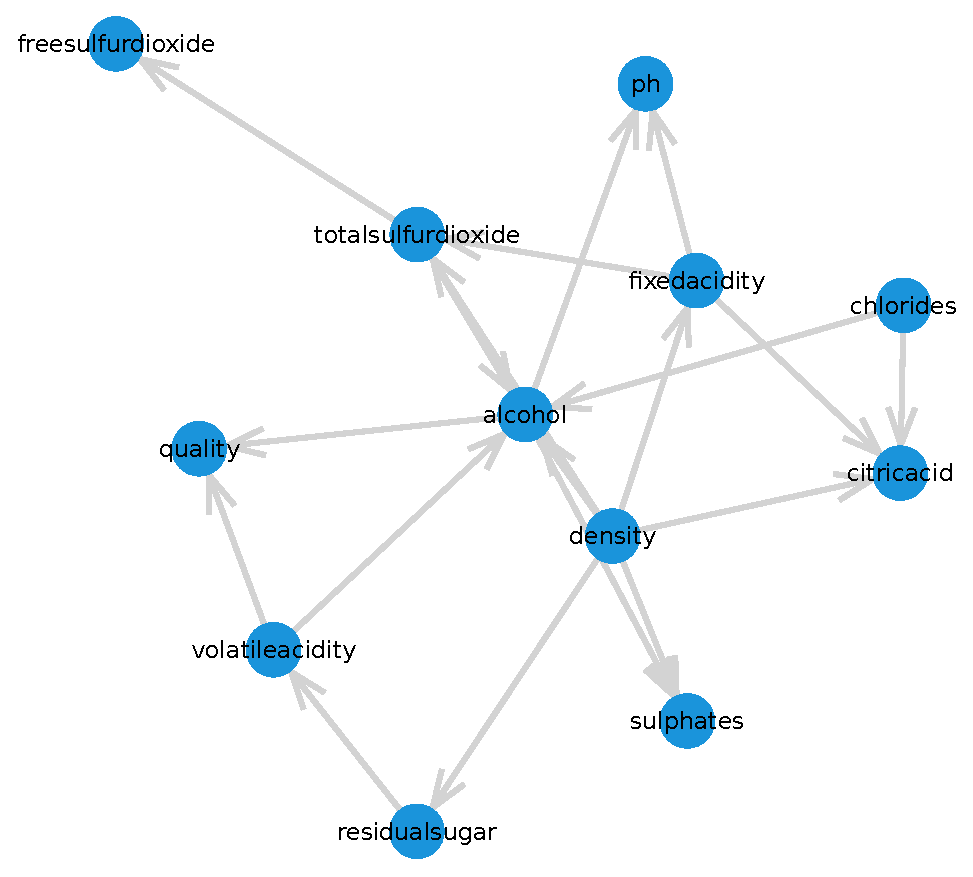
\includegraphics[height=0.33\textheight]{figs/medium-K2-100}
%		\setlength{\belowcaptionskip}{-10pt}
%		\captionof{figure}{Bayesian network learned from the \texttt{medium} dataset (12 variables) using a K2 search of the space of directed acyclic graphs with 100 randomized starts. ($\ln P(G\mid D) \approx -41961 $)}
%		\label{fig:medium_graph}
%	\end{Figure}
%\end{multicols}

	
\end{document}